\documentclass[12pt,a4paper]{article}

% Package imports
\usepackage[utf8]{inputenc}        % Allows UTF-8 input
\usepackage{amsmath,amsfonts,amssymb} % For math symbols
\usepackage{graphicx}               % For including graphics
\usepackage{hyperref}               % For hyperlinks
\usepackage{geometry}               % Set page dimensions
\usepackage{fancyhdr}               % For custom headers/footers
\usepackage{enumitem}               % For custom lists
\usepackage{setspace}               % For line spacing
\usepackage{titlesec}               % For section formatting
\usepackage{booktabs}               % For nicer table formatting
\usepackage{array}                  % For advanced table options
\usepackage{subcaption}  % Add this to your preamble
\usepackage[
backend=biber,
style=numeric,
]{biblatex}                         % For bibliography
\addbibresource{references.bib}     % Add bibliography file

% Set the margins (adjust as needed)
\geometry{
    top=1in,
    bottom=1in,
    left=1in,
    right=1in,
}

% Customizing the header and footer
\pagestyle{fancy}
\fancyhf{}
\fancyfoot[C]{\thepage}             % Centered page number

% Section title formatting
\titleformat{\section}{\large\bfseries}{\thesection}{1em}{}
\titleformat{\subsection}{\normalsize\bfseries}{\thesubsection}{1em}{}

% Set line spacing
\setstretch{1}

% Title and author (can be customized as needed)
\title{Decision Tree Classifier for Iris Dataset}
\author{Leihan Chen}
\date{\today}

% Document starts here
\begin{document}

% \maketitle

% Introduction section
\section{Introduction}
The report mainly addresses the task to apply a decision tree classifier to the Iris dataset\cite{iris_53}. Section \ref{sec:dataset}
provides information on the description of Iris dataset. 
Section \ref{sec:methodology} describes the pre-processing of the dataset, 
as well as the setting of decision tree classifier in a nested cross validation setting. 
Section \ref{sec:results} presents the results of the classifier. Finally, Section \ref{sec:conclusion} concludes the report. 


% Dataset section
\section{Dataset}\label{sec:dataset}
Iris dataset is a well-known small dataset for testing classification algorithms. It contains 150 samples of iris flowers, each with four features: sepal length, sepal width, petal length, and petal width. 
The goal is to classify each sample into one of three species: setosa, versicolor, or virginica. The dataset is balanced, with 50 samples for each species. 
A visualization of individual features is shown in figure \ref{fig:iris_features_distribution}.
It is clearly observed that the petal length and petal width have a strong correlation with the target class. 
While figure \ref{fig:iris_boxplot} shows the box plot of each feature, which indicates that the sepal width has a few outliers while all other features are distributed without obvious outliers.

% Methodology section
\section{Methodology}\label{sec:methodology}
\subsection{Pre-processing}\label{subsec:preprocessing}
Through the visualization of the dataset, very few outliers are observed. Therefore, a simple 3 standard deviation rule is applied to remove the outliers.
However, considering normalization is not necessary for decision tree classifier, no normalization is applied to the dataset. 
PCA\cite{MACKIEWICZ1993303} is also considered to the dataset to reduce the dimensionality.
Considering Iris dataset only contains four feature and they are not highly correlated so it is not applied finally.
\subsection{Decision Tree Classifier}\label{subsec:classifier}
To optimize the hyperparameters of the decision tree classifier (max\_depth, min\_sample\_split), a nested cross-validation\cite{scikit-learn_cross_validation} is applied. 
Specifically, the outer loop is a 10-fold cross-validation, and the inner loop is a 4-fold cross-validation for finding the best hyper parameters. 
The final report accuracy is the average accuracy of the outer loop and we get the feature importance of the decision tree classifier.


% Results section
\section{Results}\label{sec:results}
Through nested cross-validation, the average accuracy of the decision tree classifier is 0.947 while the standard deviation is 0.050. 
A visualization of best parameters for each outer fold is shown in figure \ref{fig:best_parameters}. We can observe that the best max\_depth range is [2, 5] and the best min\_sample\_split range is [2, 7]. 
The feature importance of the decision tree classifier is shown in figure \ref{fig:feature_importance}. 
It is clearly observed that petal width contributes most (0.858) for classification and petal height contributes average 0.147 while other two features almost have no contribution to the classifier, which is consistent with the visualization of the dataset.

\section{Conclusion}\label{sec:conclusion}
In summary, a decision tree classifier is applied to the Iris dataset with a nested cross-validation setting. Outliers in the dataset is removed while no normalization is applied. The final accuracy achieves 0.947 with a standard deviation of 0.050. 
The low standard deviation indicates that the classifier is stable. The feature importance of the decision tree classifier suggests that petal length and petal width are the most important features for classification.

% References section
\printbibliography
% Alternatively, for manually added references, comment the above lines and use:
% \begin{thebibliography}{99}
% \bibitem{ref1} Author, Title, Journal, Year.
% \bibitem{ref2} Author, Title, Journal, Year.
% \end{thebibliography}
\section{Appendix}\label{sec:appendix}
\begin{figure}[h]
    \centering
    \begin{subfigure}{0.48\textwidth}
        \centering
        % set two figures height identical
        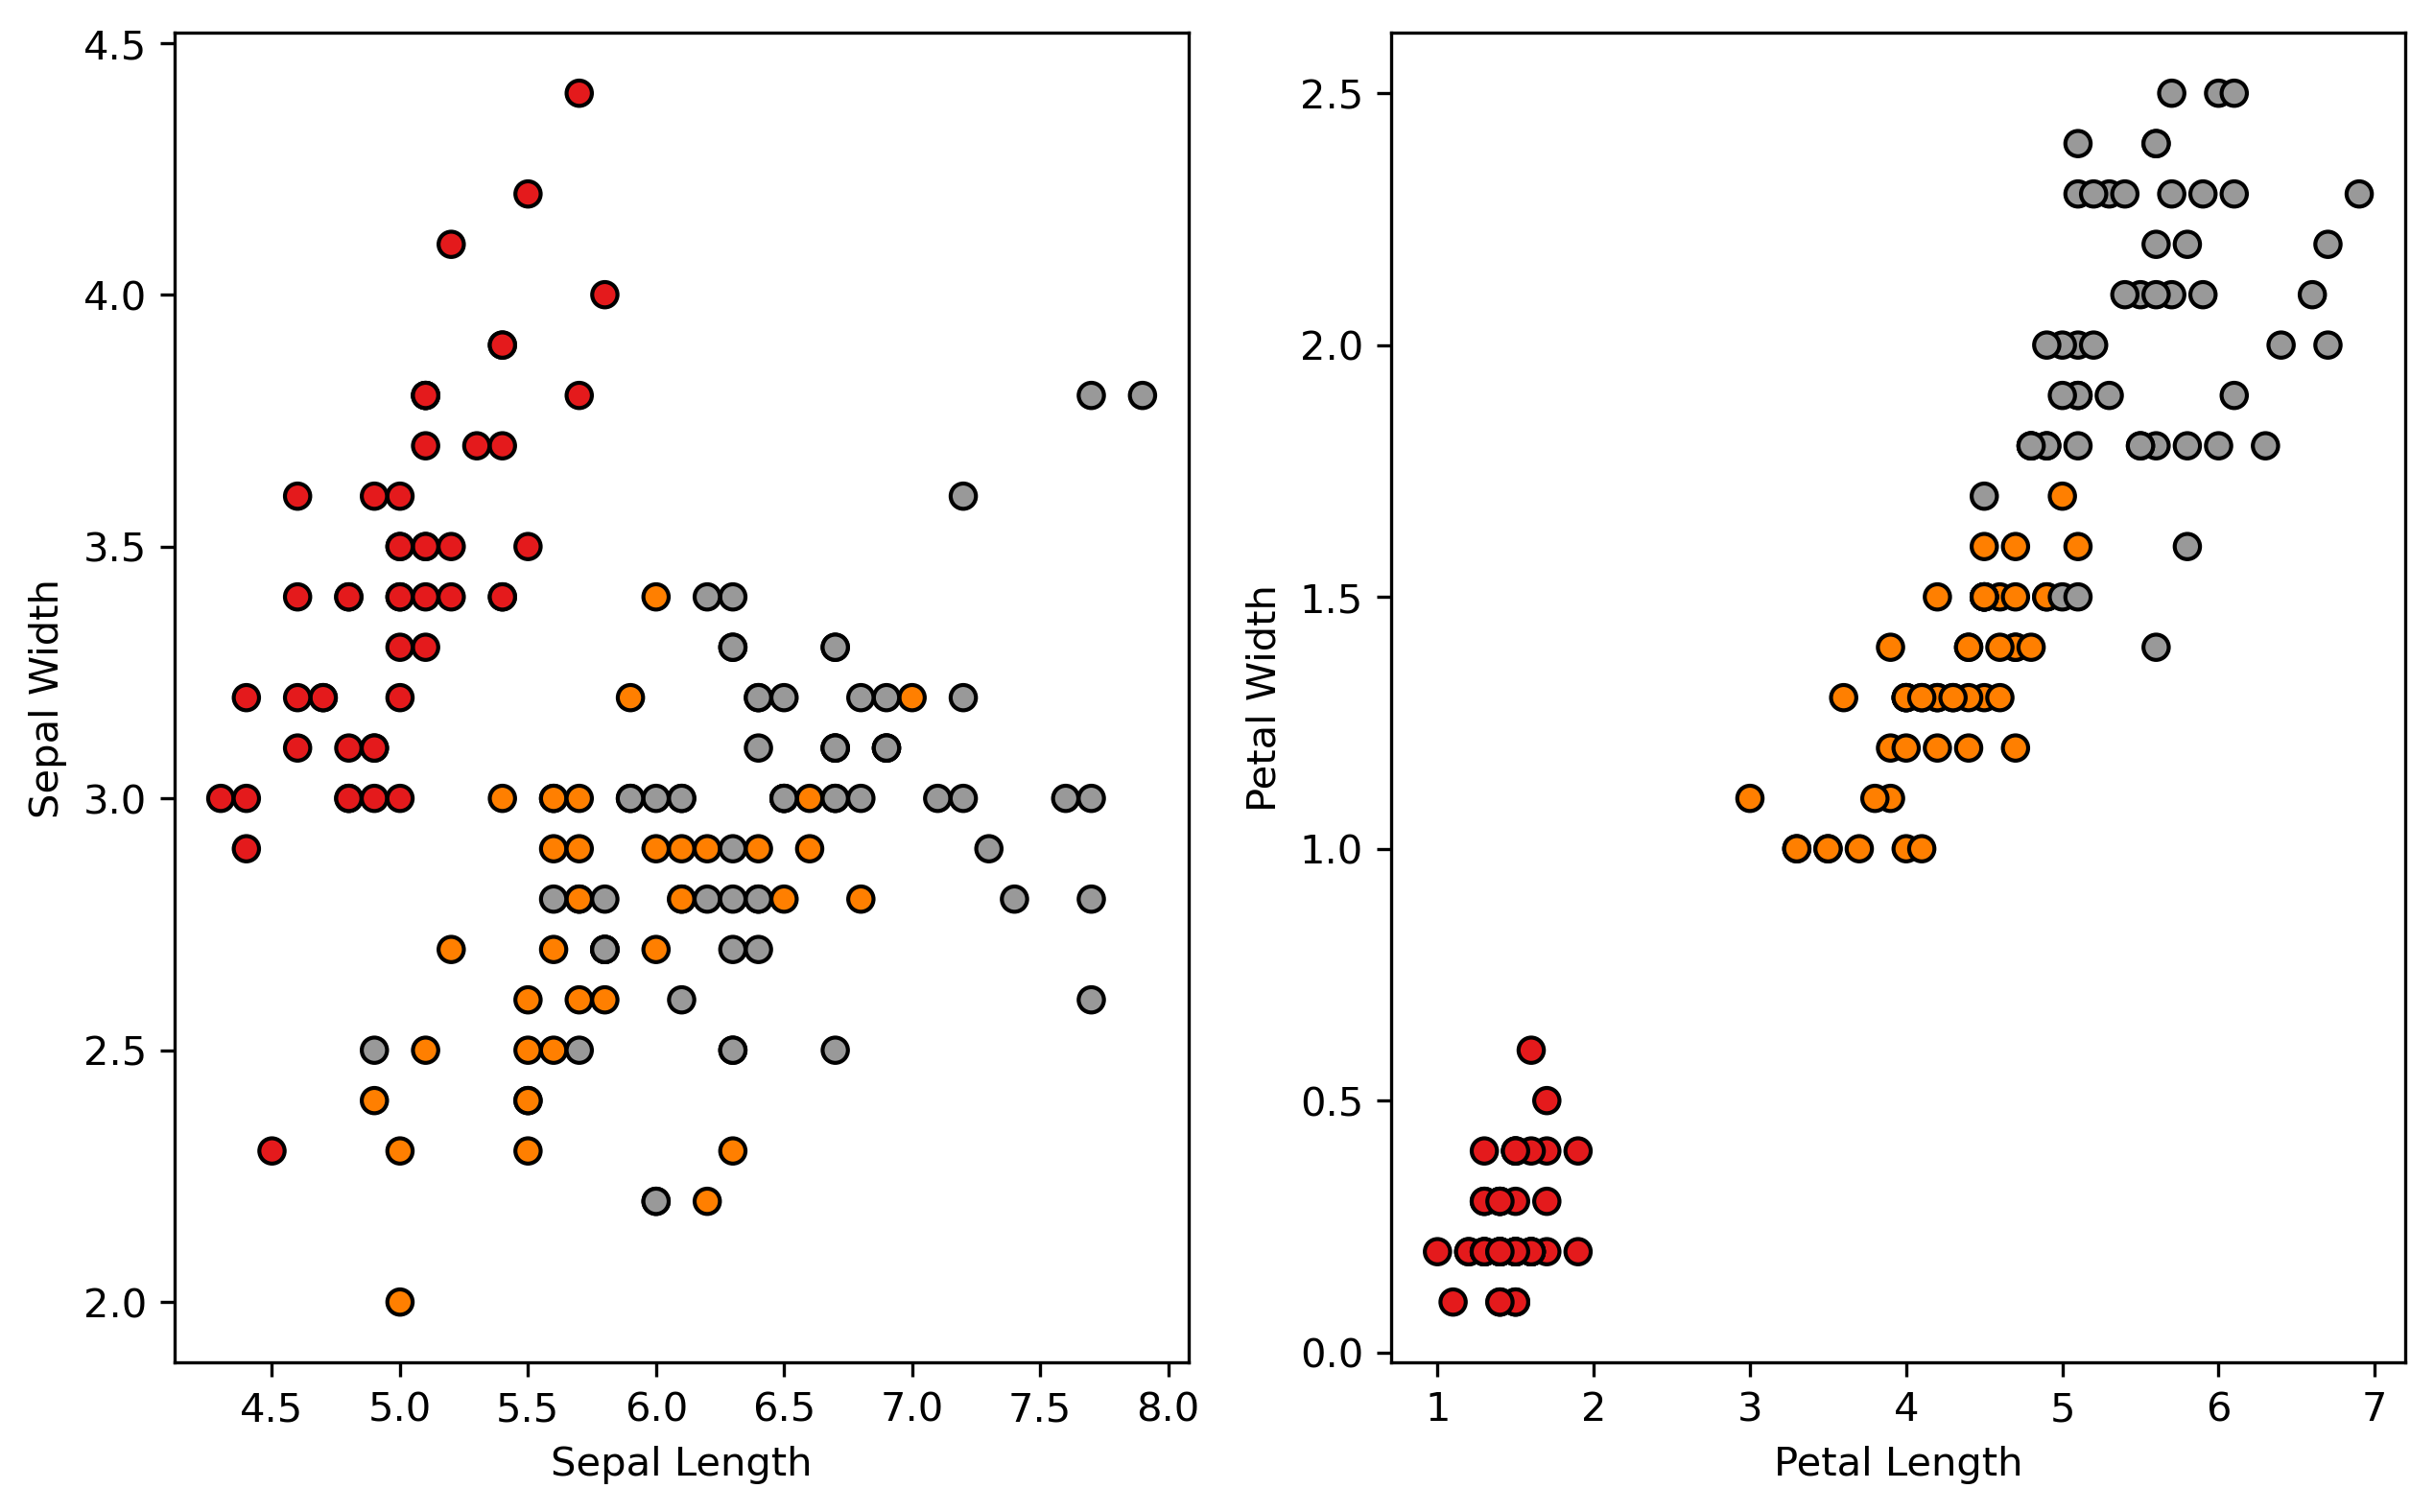
\includegraphics[width=\linewidth, height=4cm]{figures/iris_feature.png}
        \caption{Iris features distribution}
        \label{fig:iris_features_distribution}
    \end{subfigure}
    \hfill
    \begin{subfigure}{0.48\textwidth}
        \centering
        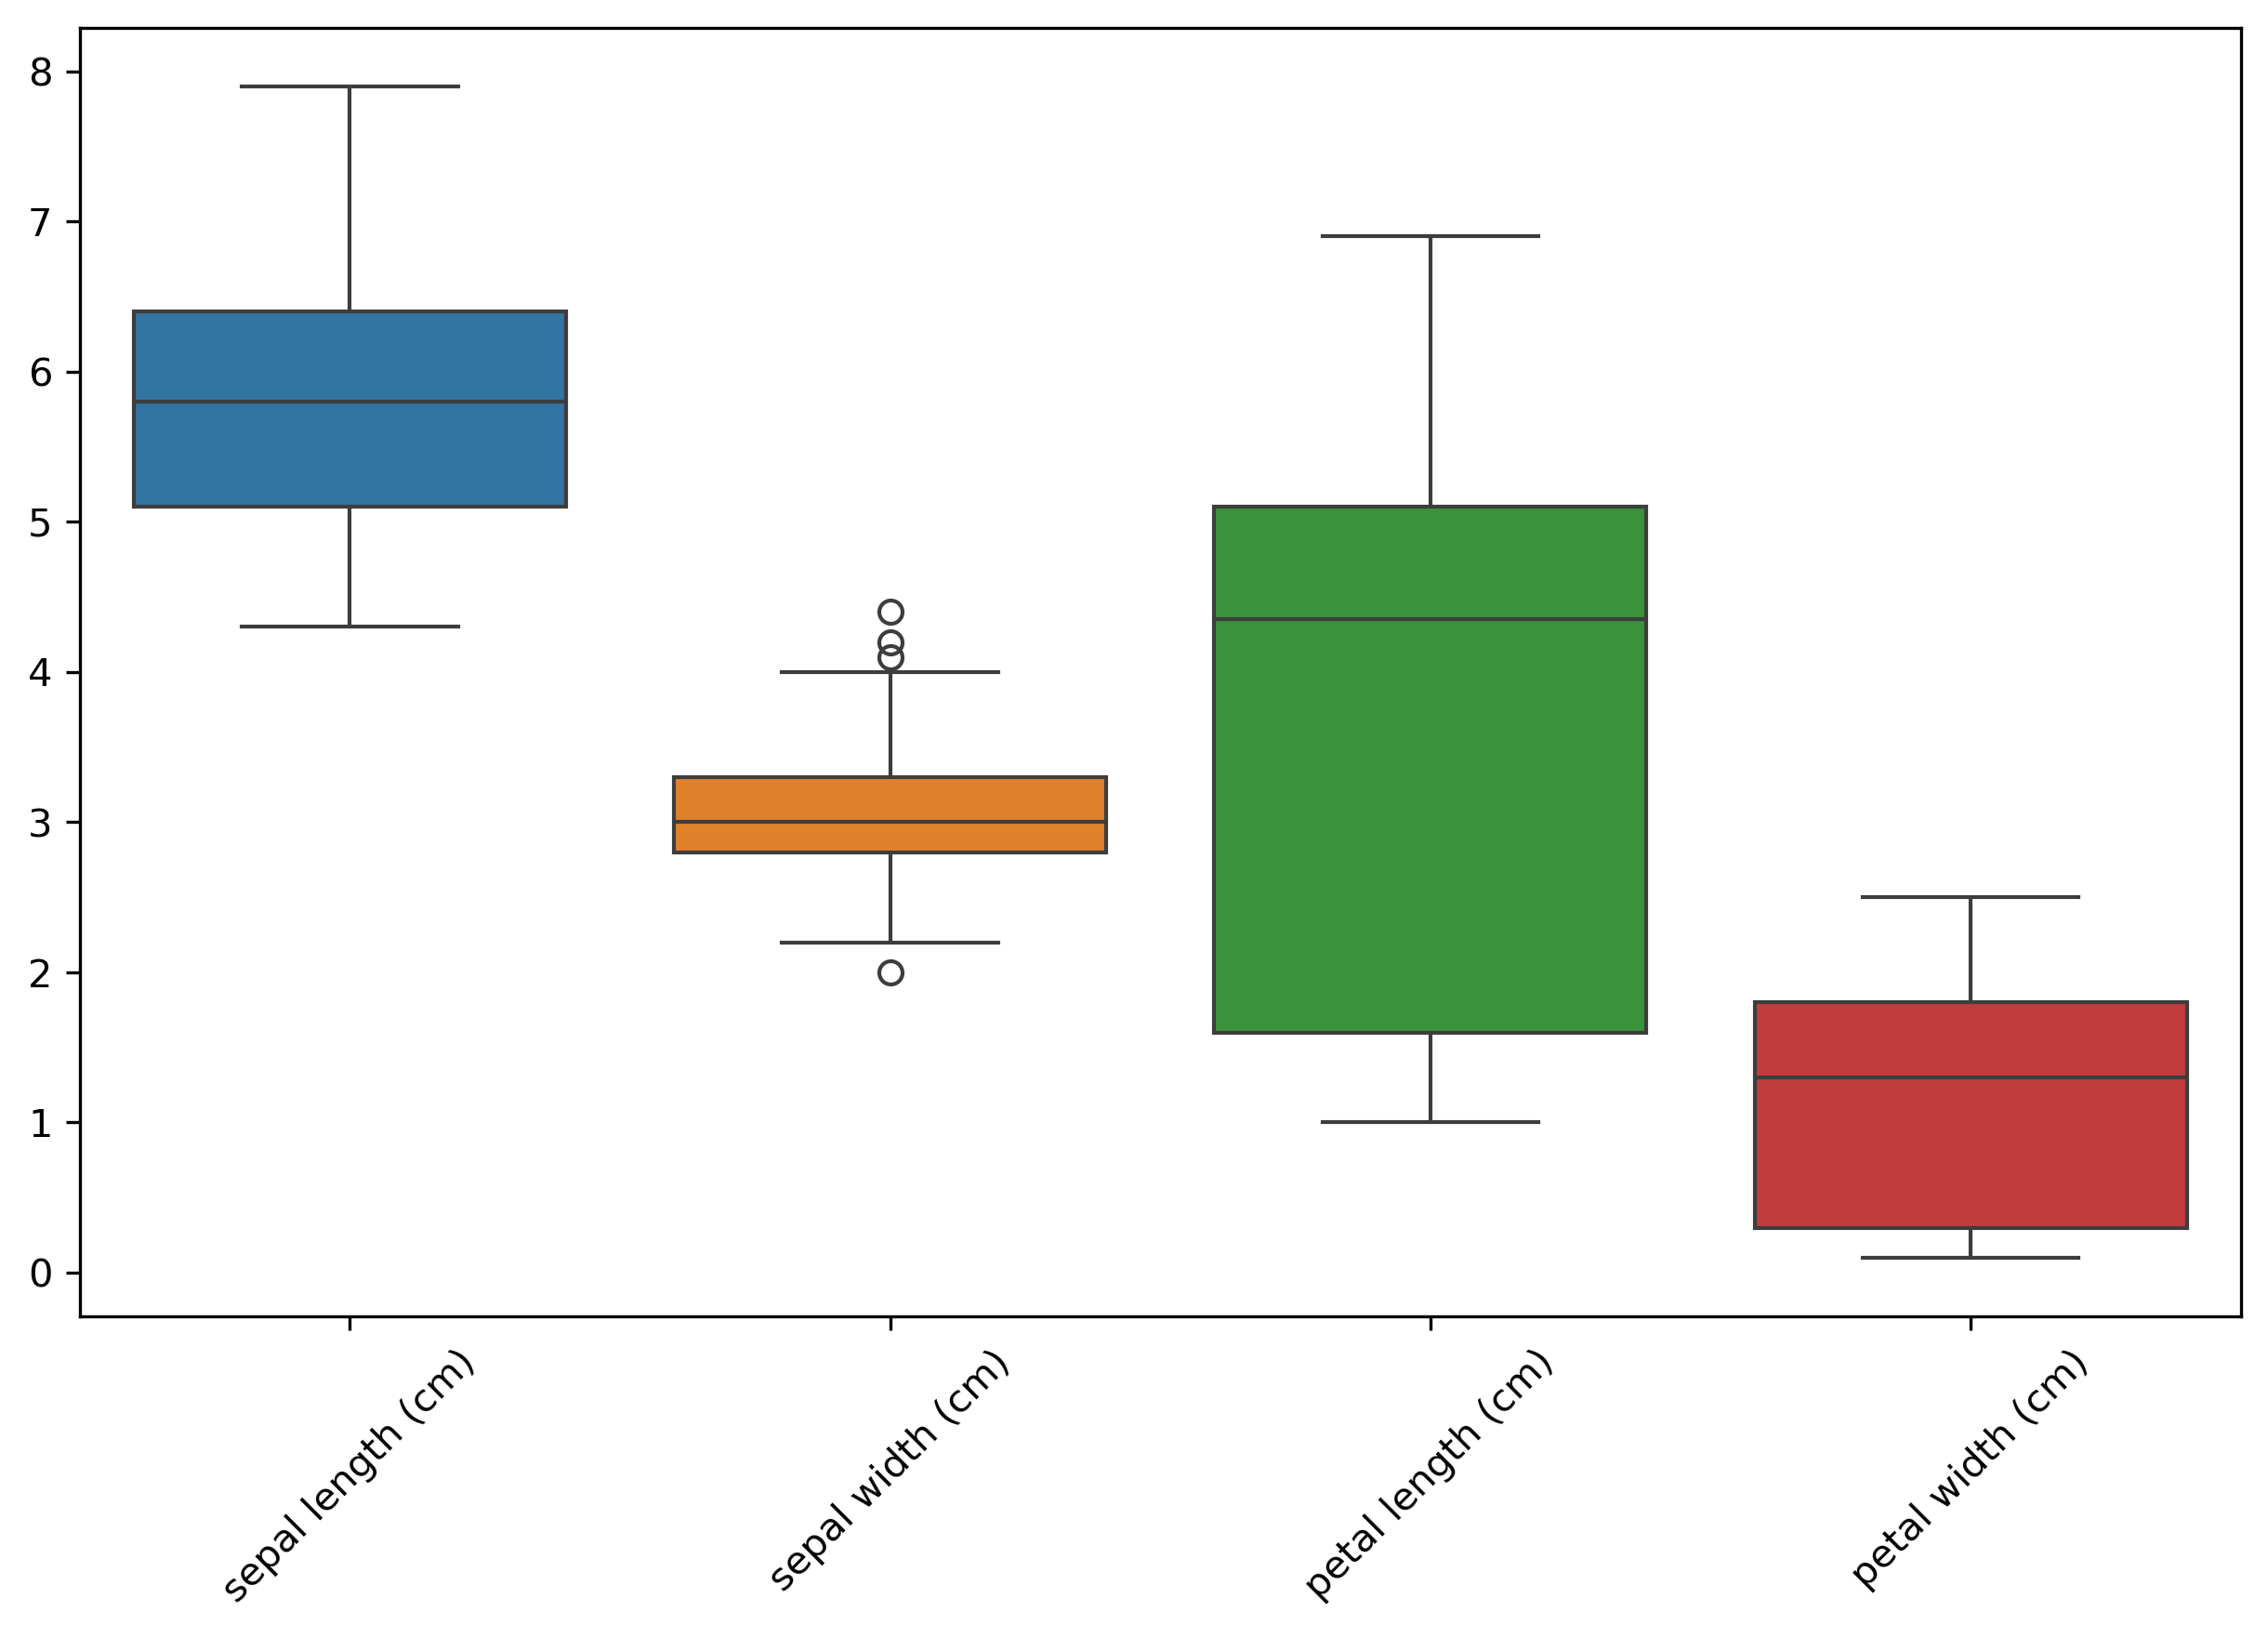
\includegraphics[width=\linewidth, height=4cm]{figures/iris_boxplot.png}
        \caption{Box plot of Iris features}
        \label{fig:iris_boxplot}
    \end{subfigure}
    \caption{Four features of Iris dataset}
    \label{fig:iris_features}
\end{figure}

\begin{figure}[h]
    \centering
    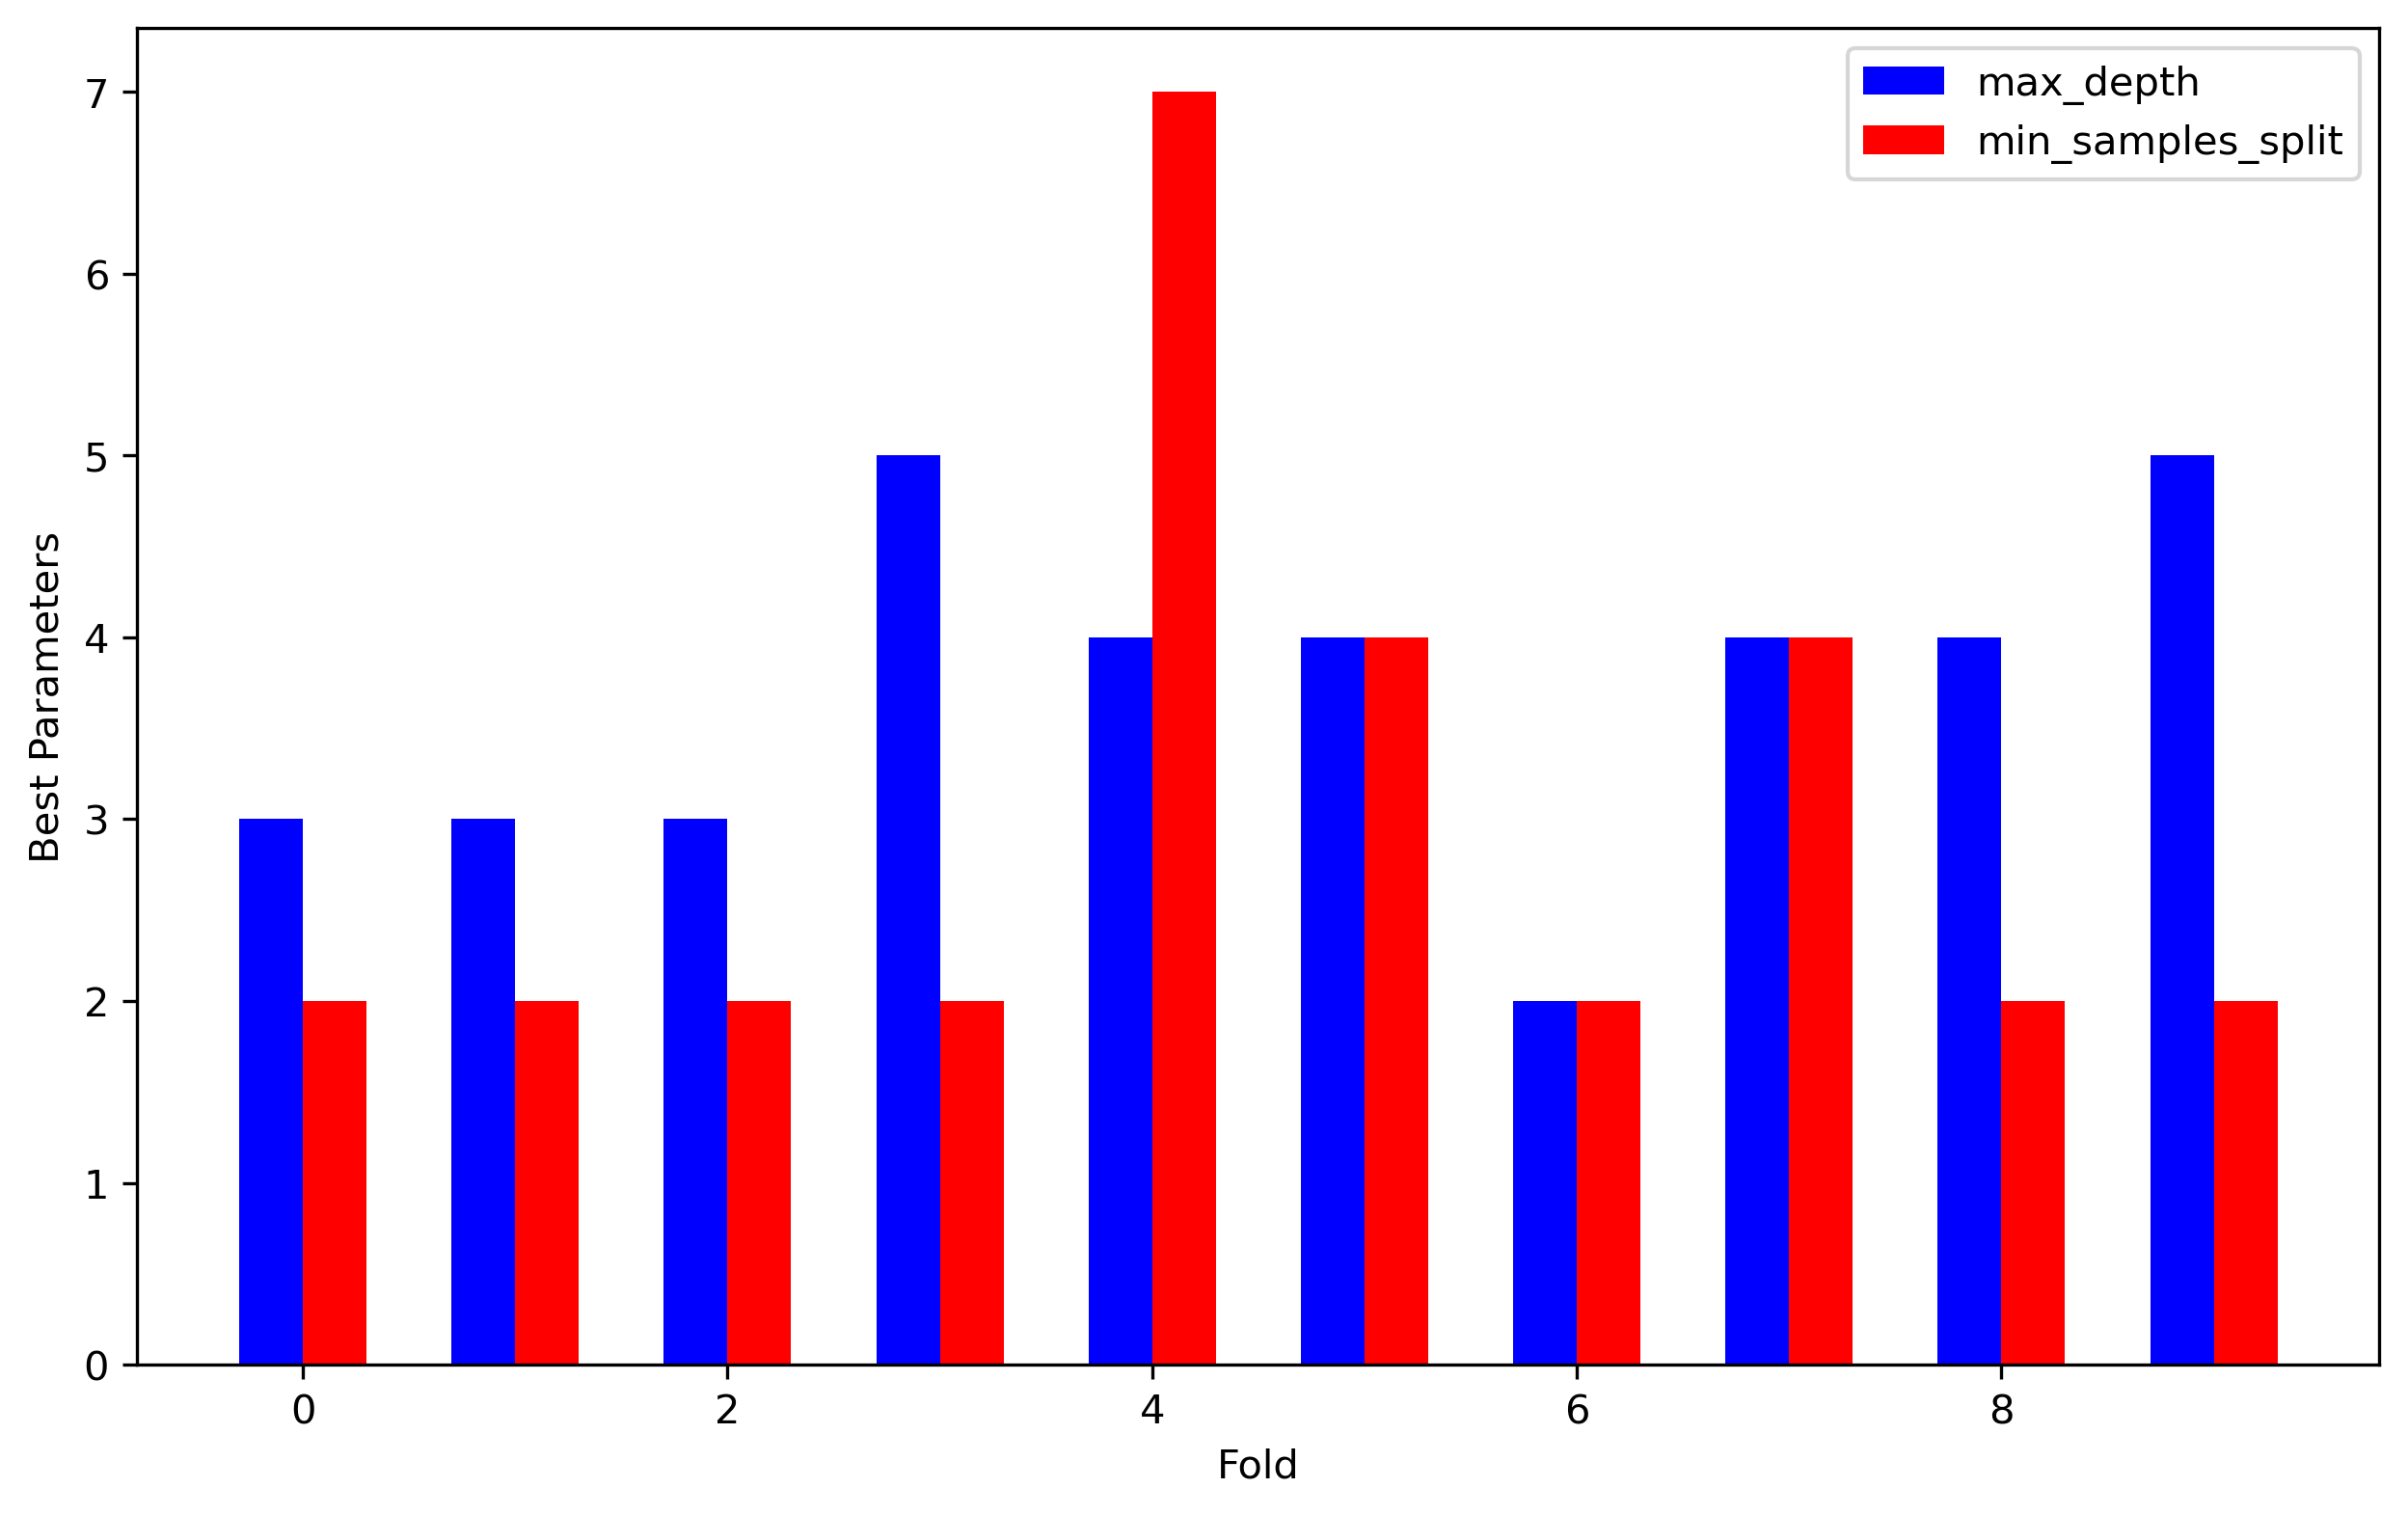
\includegraphics[width=0.8\textwidth]{figures/iris_best_parameters_for_each_fold.png}
    \caption{Best parameters for each outer fold}
    \label{fig:best_parameters}
\end{figure}

\begin{figure}[h]
    \centering
    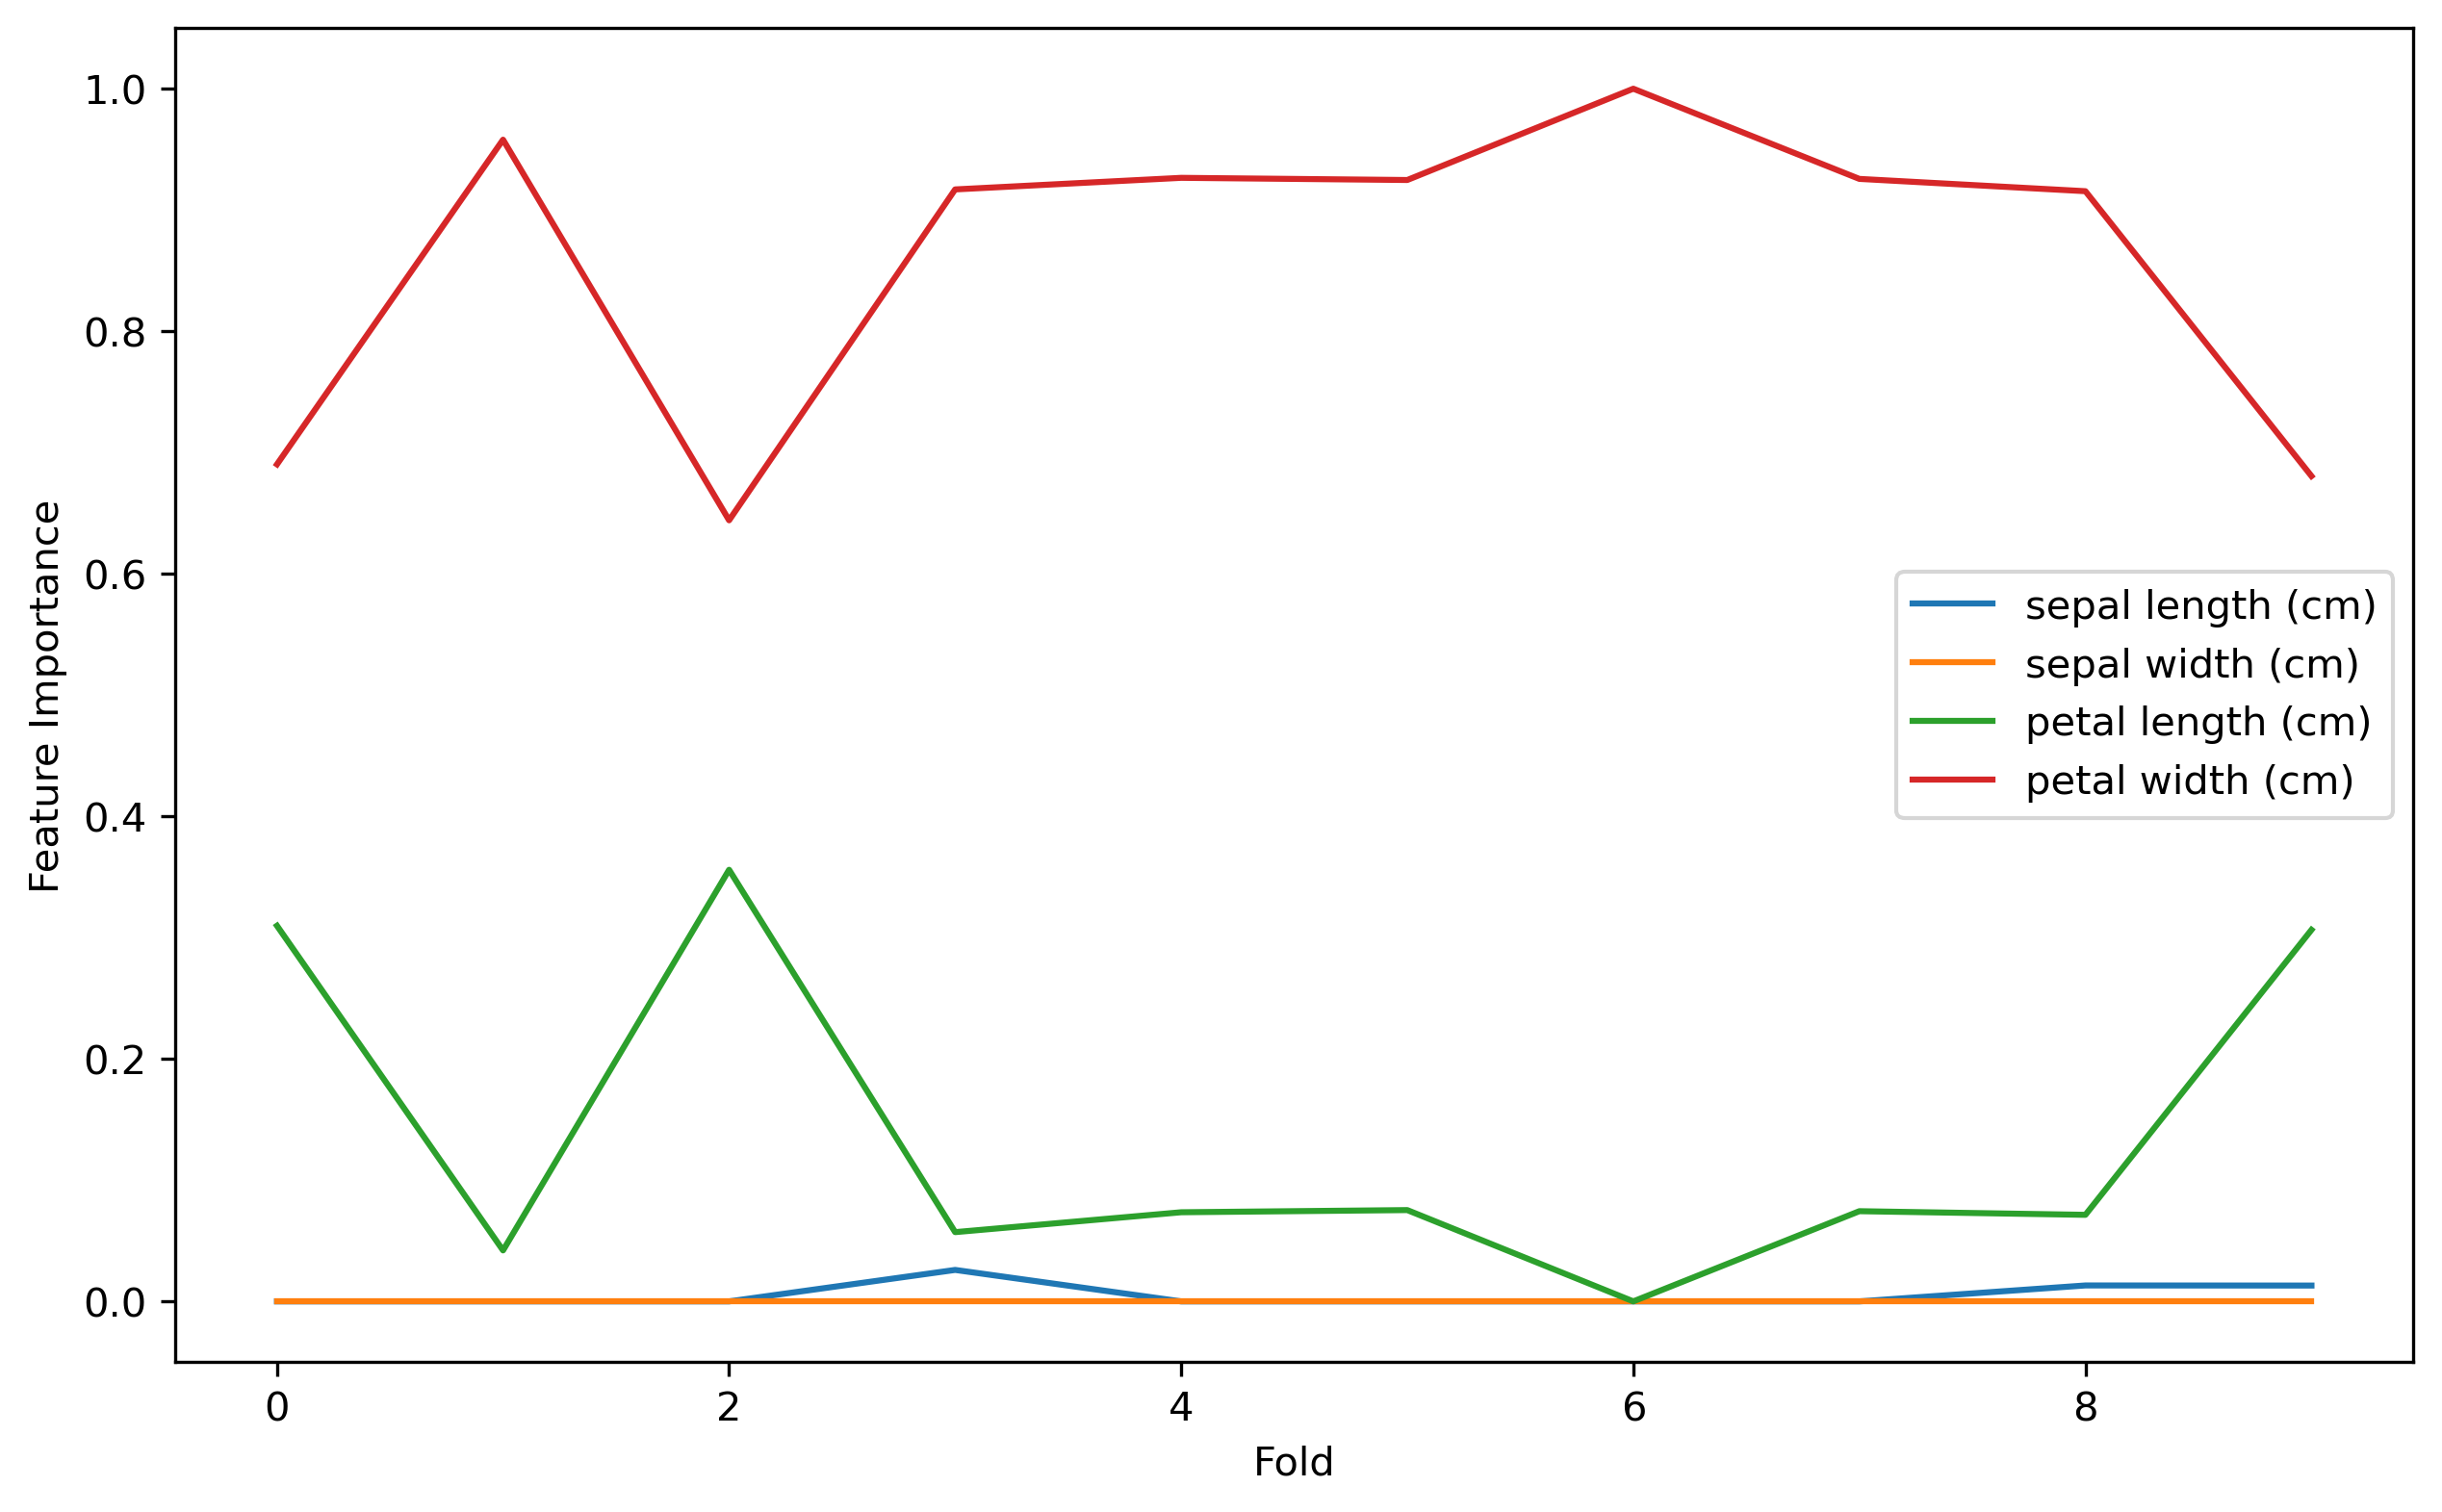
\includegraphics[width=0.8\textwidth]{figures/iris_feature_importance_for_each_fold.png}
    \caption{Feature importance of decision tree classifier}
    \label{fig:feature_importance}
\end{figure}

\end{document}